\chapter{Phase de développement~: implémentation d'un module statistique}
	\paragraph{}
	Nous avons maintenant une idée précise de ce a quoi devra ressembler le module
	statistiques, il nous faut à présent le développer.
	
	\subsection{Une gestion de projet en mode agile}
		\paragraph{}
		Introduction de la sous partie.
		
		\subsubsection{Une méthodologie qui s'inspire des méthodes agiles}
			\paragraph{}
			
			\begin{figure}[H]% Méthodo de la conception
				\centering
				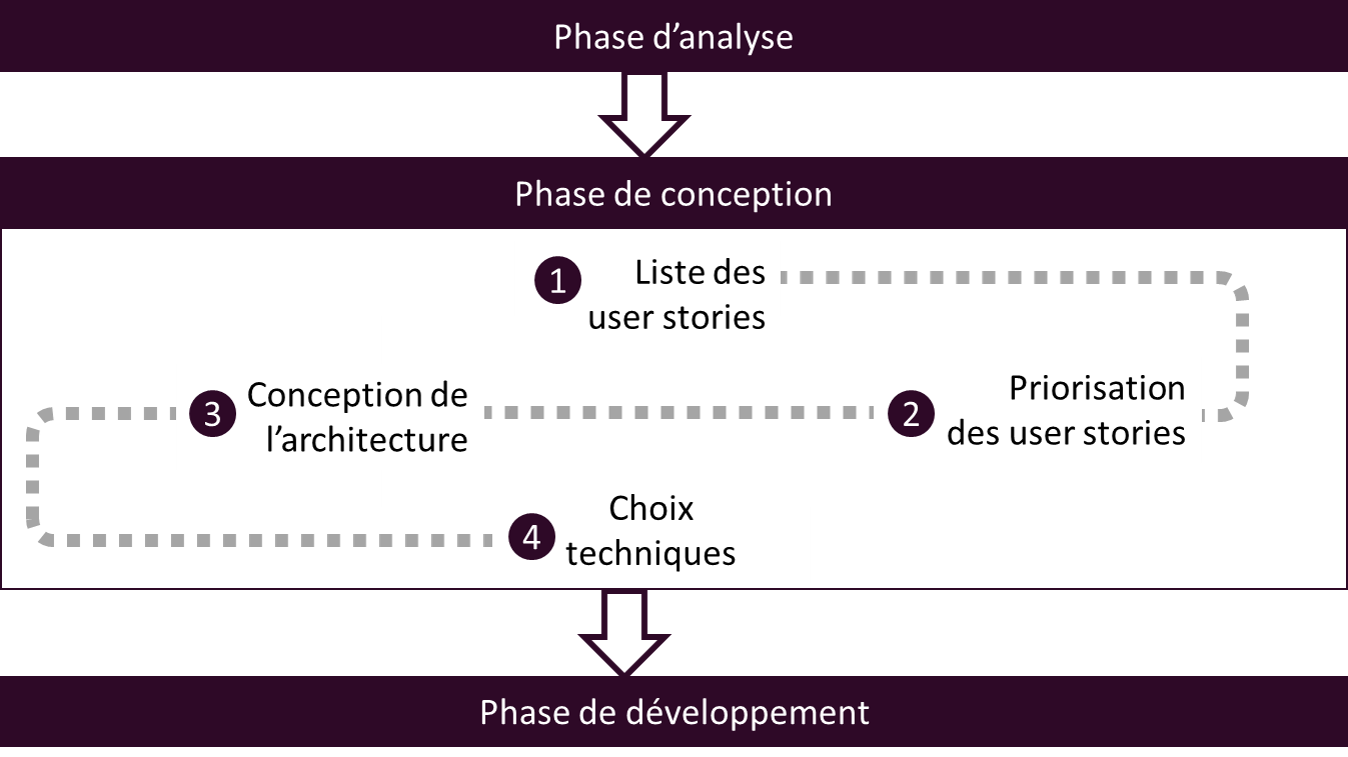
\includegraphics[width=15cm]{../img/part3/methodo_conception.png}
				\caption{\label{methodo_conception} Méthodologie de la conception du
				nouveau module.}
			\end{figure}
			
			\begin{figure}[H]% Méthodo du dééveloppement
				\centering
				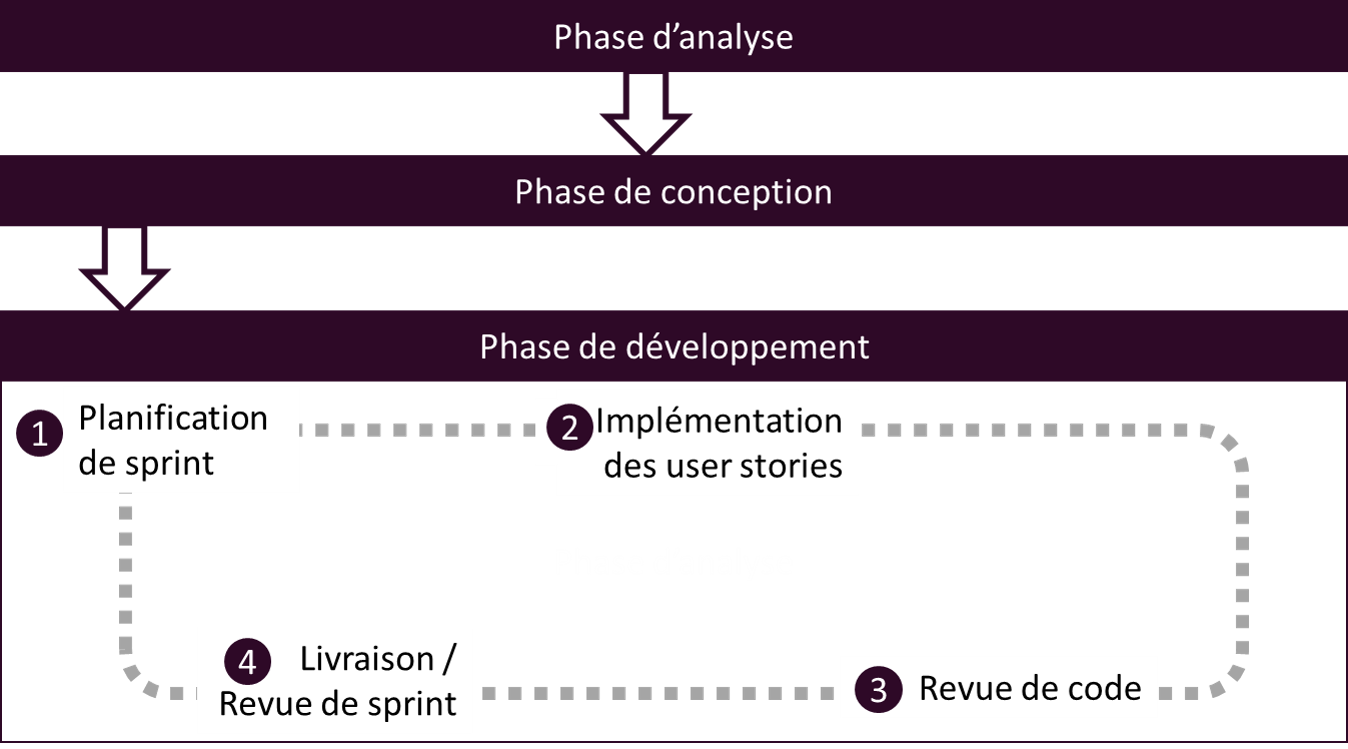
\includegraphics[width=15cm]{../img/part3/methodo_dev.png}
				\caption{\label{methodo_dev} Le développement se déroule en sprints de
				deux semaines chacun.}
			\end{figure}
		
		\subsubsection{Élaboration du backlog}
	
	\subsection{TrackCIS, une application web en deux parties}
		
		\subsubsection{Qu'est-ce qu'une application web ?}
			\paragraph{}% Modèle client serveur classique
			TrackCIS est une application accessible depuis un navigateur internet, il
			s'agit d'une application web. TrackCIS est installé au niveau d'un serveur,
			généralement citué au sein de l'établissement hospitalier et connecté au
			réseau local. La machine de l'utilisateur, que l'on appel le client, ce
			connecte à ce serveur. Ce dernier reçoit de la part du client une requête
			HTTP (protocole standard d'échange sur internet).
			
			\paragraph{}% Modèle AJAX
			
		\subsubsection{TrackCIS est composé d'un frontal et d'une API}
			\paragraph{}% Archi générale de l'application
			
			\begin{figure}[H]% Architecture globale de l'application
				\centering
				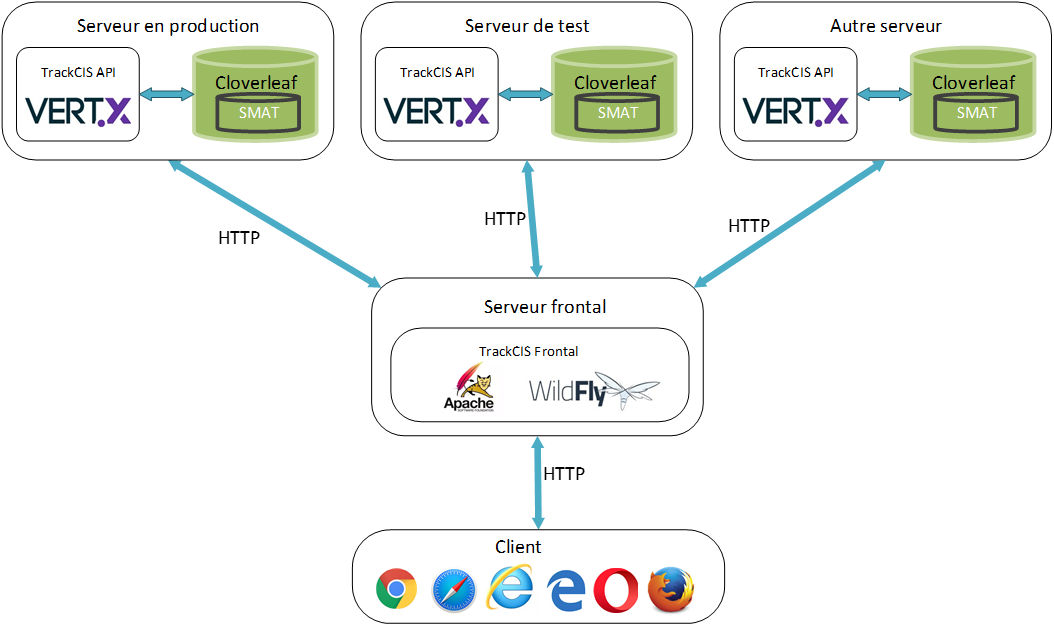
\includegraphics[width=10cm]{../img/part3/archi_trackcis.png}
				\caption{\label{archi_trackcis} TrackCIS est composés de deux éléments
				distincts pouvant se trouver sur des serveurs différents.}
			\end{figure}
			
		\subsubsection{Le frontal est développé en java J2EE}
			\paragraph{}% Les bases de la POO
			
			\paragraph{}% les grandes lignes de l'archi du front
			
		\subsubsection{L'API permet de communiquer avec Cloverleaf}
			\paragraph{}% Les grandes lignes de l'archi de l'API
	
	\subsection{L'analyse technique permet d'implémenter le nouveau module sur
	l'existant}
		\paragraph{}
		Introduction de la sous partie.
		
		\subsubsection{Un module qui est basé sur les données disponibles dans
		Cloverleaf}
		\subsubsection{Nouvelle architecture de l'application}
			\paragraph{}% Une archi dessinée à partir des contraintes fonctionnelles
			Le module statistique de TrackCIS doit :
			\begin{itemize}% Liste des contraintes
			  \item être basé sur l'architectture déjà en place. Il n'est pas question
			  dans ce projet de faire de grosses modifications sur l'existant. Ceci est
			  valable aussi bien pour le code lui-même que pour la structure de la base
			  de donnée.
			  \item être fermé à la modification et ouvert à l'extention. C'est-à-dire
			  qu'il doit être possible, pour une équipe de développement ultérieur,
			  d'ajouter des fonctionnalités au module sans ajour à modifier le code
			  existant.
			  \item ne pas perturber le fonctionnement de Cloverleaf. Pour afficher des
			  données pertinentes pour l'utilisateur, certains traitements seront
			  nécessaires sur les données brutes. Ceux-ci peuvent cependant ralentir ou
			  perturber le fonctionnement de Cloverleaf. Il est nécessaire pour cela que
			  ces traitements ne soient pas fait sur le serveur de l'EAI, donc pas au
			  niveau de l'API.
			  \item ne pas surchager le serveur sur lequel est déployé le frontal. Le
			  serveur servant à héberger le frontal n'est pas forcément une machine très
			  puissante, bien que cela varie en fonction des établissements.
			\end{itemize}
			
			\begin{figure}[H]
				\centering
				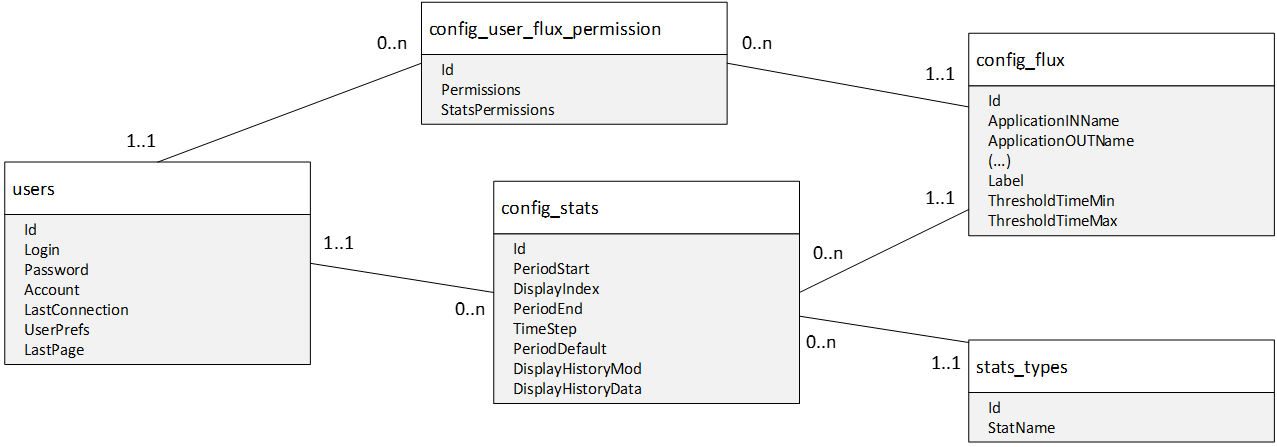
\includegraphics[width=16cm]{../img/part3/modele_donnee.png}
				\caption{\label{modele_donnee} Le nouveau modèle de donnée de TrackCIS au
				niveau du frontal.}
			\end{figure}
			
		\subsubsection{Réalisation des choix techniques}
			\paragraph{}% Liste des choix
			Le développement de ce projet implique l'utilisation d'un certain nombre de
			technologies. Certaines d'entre elles n'ont pas été utilisée pour le
			développement de la première version de TrackCIS.
			Le tableau ci-dessous résume l'ensemble des technologies qui ont été
			utilisées pour le développement de TrackCIS jusqu'a présent (c'est-à-dire
			avant le présent travail).
			
			\paragraph{}% Méthodo des choix
			Nous n'allons pas ici détaillé tous les choix techniques qui ont été fait.
			Nous mettrons en avant dans cette partie la méthodologie avec laquelle ces
			différents choix tecnique on été effectué en l'illustrant d'un exemple, en
			l'occurence le choix de la bibliothèque graphique javascript. Comme nous
			l'avons vu dans l'architecture de nouveau module, les graphiques sont
			dessinés par le navigateur client. La navigateur reçois un ensemble de script
			javascript qu'il sait interpréter. Certains de ces scripts permettrons donc
			d'afficher les graphiques. Pour cela nous avons besoin d'une bibliothèque
			javascript, c'est-à-dire un ensemble de fonctions précrites. Il en existe de
			très nombreuses et certaines sont gratuites et libres. Pour faire notre choix
			nous partons des contraintes suivantes :
			\begin{itemize}
			  \item La bibliothèque doit être gratuite et son utilisation pour la
			  création de produits commerciaux doit l'être également.
			  \item Elle doit permettre à minima de dessiner les types de graphiques
			  spécifiés dans les fonctionnalités (courbe et historgamme avec plusieurs
			  séries de données, jauge et donut).
			\end{itemize}
			% Listing des librairies qui répondent à ces critères
			
			% Listing des autres critères de choix qui ne sont pas éliminatoires
			
			% Explication du système de pondération et de notation
			
			% Bilan : on choisi d3.js
	
	\subsection{Bilan de la phase de développement et suite du projet}
		\paragraph{}
		Cette dernière partie est l'occasion de faire le bilan sur ce qui a été
		implémenté.
		
		\subsubsection{Les fonctionnalités implémentées}
			\paragraph{}
		
		\subsubsection{Un module maintenable}
			\paragraph{}% Principes et intérêts de la documentation~: plusieurs niveaux
			%  de doc
			La maintenabilité du module est facilité par :
			\begin{itemize}
			  \item la présence d'une documentation du code (ou javadoc),
			  \item la présence de tests unitaires dans le code.
			\end{itemize}
			
			\paragraph{}% documentation du code~: la java doc
			
			\paragraph{}% les tests unitaires
			
		\subsubsection{Les suites possibles du projet pour Xperis}
			\paragraph{}
			
			\paragraph{}
			